\documentclass[11pt,a4paper]{article}
\usepackage[T1]{fontenc}
\usepackage{lmodern}
\usepackage[margin=24mm]{geometry}
\usepackage{amsmath,booktabs,graphicx,tabularx}
\usepackage[hidelinks]{hyperref}
\usepackage{xcolor}

\newcommand{\teamname}{Porte}
\newcommand{\studentnames}{Walae Laamoum \\ Eldana Ashirova \\ Yomna El Nikety}
\newcommand{\projectrepo}{\url{https://github.com/yomnaelnikety/porte_deep_learning}}
\newcommand{\todo}[1]{\par\smallskip\noindent\textcolor{blue!65!black}{\textit{[To complete] #1}}\par\smallskip}

\begin{document}
\hypersetup{pageanchor=false}
\pagenumbering{gobble}
\begin{titlepage}
\centering
\vspace*{30mm}
{\Large AI2210 \textbar{} Deep Learning \& Neural Networks\par}
\vspace{15mm}
{\Huge\bfseries EventFlow\par}
\vspace{3mm}
{\LARGE Temporal Event Prediction\par}
\vspace{19mm}
{\large\bfseries \teamname\par}
\vspace{5mm}
{\large\studentnames\par}
\vfill
{\small Project repository\par\projectrepo\par}
\end{titlepage}
\pagenumbering{arabic}
\hypersetup{pageanchor=true}

\begin{abstract}
\todo{Summarize the task, best model and final test log loss, one ablation finding and one generation finding. Write this last.}
\end{abstract}

\section{Task, data and representation}
Given an observed log prefix from one machine, the model predicts a distribution over 14 next-event classes. The release contains complete histories for 6,500 training systems and truncated histories for 900 test systems \cite{brief}. Each observed row includes an event identity, timestamp, contextual fields and numerical measurements. We sort by event index within each system and form the label from the first event after the cutoff.

\IfFileExists{tables/data_summary.tex}{In the fitting split, RECOVERY is the most frequent event (26.5\%) and CONTROL\_ALERT is the least frequent (1.0\%). The median gap between consecutive events is 0.96 timestamp units and the 95th percentile is 2.93. The highest missing fraction is 1.6\% for vibration\_reading.
}{
\todo{Summarize the fitting split's class imbalance, sensor missingness and inter-event gaps using the EDA outputs.}}
\IfFileExists{figures/eventflow_eda.pdf}{
\begin{figure}[htbp]
\centering
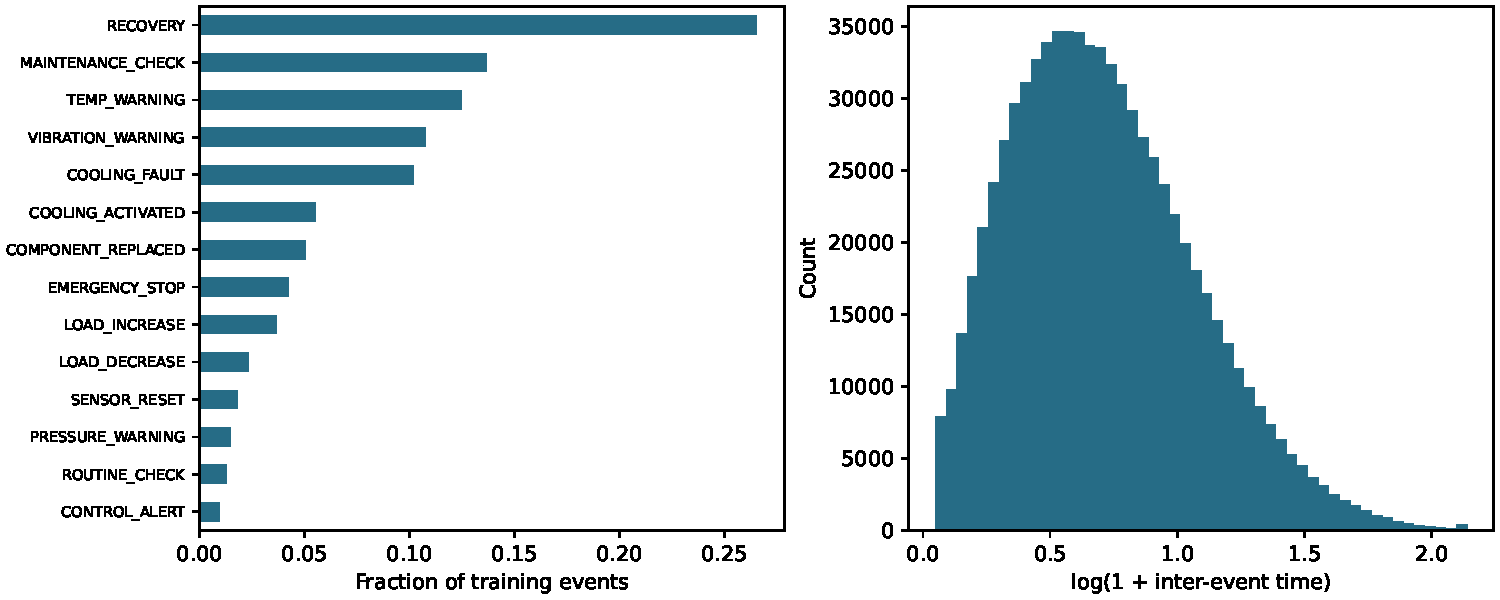
\includegraphics[width=0.88\linewidth]{figures/eventflow_eda.pdf}
\caption{Event frequency and inter-event gap distribution within fitting systems.}
\end{figure}}{}

\begin{table}[htbp]
\centering\small
\begin{tabularx}{\linewidth}{@{}lX@{}}
\toprule
Feature group & Representation and motivation \\
\midrule
Current record & Latest event, context and measurements capture the machine state at the cutoff. \\
Event order & The previous six events and the final event pair represent short transition motifs. \\
Event counts & Per-class counts over the last 8, 32 and 90 events measure recent prevalence at different scales. \\
Timing & Recent log-transformed gaps and elapsed time since each event represent bursts and recency. A type unseen in the prefix has missing recency. \\
Sensor history & Trailing means and least-squares slopes over 8 and 32 events represent levels and trends. Slopes use event positions and skip missing values. \\
\bottomrule
\end{tabularx}
\caption{Classical features grouped for ablations.}
\end{table}
The fitting split shows positive correlations between the main and secondary temperature probes ($r=0.61$) and between the vibration probes ($r=0.79$). The secondary temperature probe also changes more between successive records (median absolute change 0.090 versus 0.056). These differences suggest testing whether trailing means and slopes add information beyond a single reading. Observed variation combines actual changes in system state with possible measurement noise.

\section{Model development}
The smoothed transition table uses the last observed event. The current-row logistic regression uses one-hot category encoding and standardized numeric values, with imputation fitted on the fitting split. These baselines help measure the gain from longer histories and nonlinear features.

\subsection{Classical model}
We tune LightGBM \cite{lightgbm} on the feature groups in Table~1 with the categorical event pair excluded. The earlier ablation on these validation machines motivated this choice. The final test set remains held out. At the selected tree settings, we restore the 196-category pair in one ablation and remove the individual lags in another. We also fit on four sampled cutoffs per machine to check whether using fewer overlapping training examples changes performance. Categorical vocabularies are fitted on fitting prefixes and unknown levels are encoded as missing for prediction. Trees handle missing numerical values directly. The model is trained from scratch using the multiclass objective.

\subsection{First deep model}
% First deep model (GRU). Included from 02_models.tex.
The recurrent model reads the prefix event by event instead of a fixed summary. Each step is the concatenation of a 32-dimensional embedding of the event class, 8-dimensional embeddings of subsystem, severity, shift, operator group, device family and firmware channel, and numeric inputs: the log time gap to the previous event, the position in the log, all 16 measurements (including the four telemetry channels the classical sensor history omits) and a missing-value flag for each. Measurements are standardized with means and deviations from the fitting machines, and missing values are set to zero so that the flag carries the information. A linear layer with ReLU maps each step to $h$ units, a unidirectional GRU or LSTM processes the sequence, and layer normalization and a linear head give 14 logits at every step.

The recurrence only moves forward in time, so the output at step $t$ depends on events $0,\dots,t$ and is the prediction for a prefix of length $t+1$. We use this in two ways. First, training is many-to-many: one pass over a fitting machine supervises every step whose prefix length lies in 90--250, giving about 95 targets per machine per epoch instead of 12 sampled cutoffs. The classical cutoff ablation, where four instead of twelve cutoffs per machine raised log loss by 0.035, suggests that more training prefixes help. Second, variable prefix lengths need no packing. Shorter sequences are padded on the right, padding cannot affect earlier outputs, and we read the output at the last observed event. For the short-context ablation the model instead sees a random chunk of $K+32$ events and is trained only on steps with at least $K$ events of history, matching the $K$ events it receives at evaluation.

Training minimizes cross-entropy, which equals log loss, with AdamW (weight decay $10^{-4}$), batches of 64 machines and gradient-norm clipping at 1. The learning rate halves when the early-stop loss stops improving, and training stops after four epochs without improvement or after 40 epochs. We keep the weights from the best epoch. The early-stop loss is computed on the 12 manifest cutoffs of the 520 early-stop machines, so it mirrors the validation task. We then fit one temperature $T$ on the 520 calibration machines by minimizing the log loss of $\mathrm{softmax}(z/T)$. Dividing all logits by $T$ preserves their order, so accuracy is unchanged and only confidence is adjusted.


\subsection{Second deep model}
\todo{Person C. Document the architecture, temporal context, training settings and comparison to the first deep model.}

\section{Validation and optimization}
We use an 80/20 split by system ID with seed 2210. Cutoffs are sampled from lengths 90 through 250 subject to the availability of a next event. The outer training partition supplies 12 distinct cutoffs per machine. Validation uses eight fixed cutoffs per held-out machine, giving 10,400 predictions across 1,300 machines. The models use a common validation manifest and class order. We measure the mean negative natural logarithm of the assigned true-class probability,
\[
  \mathcal{L}=-\frac{1}{N}\sum_{i=1}^{N}\log p_i(y_i).
\]
Within the 5,200 outer training machines, we fit the classical model on 4,160 machines, tune and early stop on 520, and fit and select a calibration method on a separate 520. We test regularized trees with a learning rate of 0.04 and 7, 15 or 31 leaves. All feature and cutoff-count ablations fix the selected tree settings and number of boosting rounds. Calibration variants use the same raw tree probabilities. Temperature scaling applies a softmax to the log probabilities divided by a fitted temperature. Prior blending interpolates the raw predictions with a smoothed calibration-set class prior.

For each ablation, we compute paired differences in log loss on matching cutoffs and resample 1,300 machines with replacement 5,000 times, retaining all their cutoffs. The 2.5th and 97.5th percentiles give the interval. The experiment log records the protocol version and preserves the original runs. The team reserves the provided test labels for final evaluation.

If the classical pipeline is chosen for final testing, the prediction command refits the tree on all 6,500 labeled machines using the fixed cutoffs from both local splits and the selected number of rounds. The refit excludes the event pair and applies the selected calibration method. Any calibration parameters were estimated during development on the separate 520-machine calibration set using predictions from the tree trained on 4,160 fitting machines. Their effect after transfer to the refit is unverified.

\todo{List each deep model's tuning search, checkpoint criteria, calibration data and final refit protocol.}

\section{Results, ablations and errors}
\IfFileExists{tables/classical_results.tex}{\begin{table}[htbp]
\centering\small
\begin{tabular}{@{}lr@{}}
\toprule
Run & Validation log loss \\
\midrule
uniform & 2.6391 \\
markov & 1.7708 \\
current\_row\_logreg & 1.7227 \\
full\_raw & 1.5194 \\
selected\_classical & 1.5193 \\
\bottomrule
\end{tabular}
\caption{Classical results on the shared v2 cutoffs.}
\end{table}
}{
\todo{Insert the classical validation table from the experiment log.}}
\todo{Add deep model validation results and the chosen model's final test result. The brief's reference scores were measured on test and should be labeled separately from local validation.}

\IfFileExists{tables/classical_ablations.tex}{\begin{table}[htbp]
\centering\small
\begin{tabular}{@{}lrrr@{}}
\toprule
Run & Log loss & $\Delta$ vs. raw & 95\% paired CI \\
\midrule
drop\_lags & 1.5274 & +0.0080 & [+0.0048, +0.0112] \\
drop\_counts & 1.5383 & +0.0189 & [+0.0154, +0.0223] \\
drop\_time & 1.5374 & +0.0180 & [+0.0141, +0.0218] \\
drop\_sensors & 1.5219 & +0.0024 & [-0.0005, +0.0055] \\
add\_pair\_back & 1.5413 & +0.0219 & [+0.0169, +0.0269] \\
four\_fit\_cutoffs & 1.5539 & +0.0345 & [+0.0293, +0.0395] \\
temperature & 1.5193 & -0.00011 & [-0.00020, -0.00001] \\
\bottomrule
\end{tabular}
\caption{Ablations against the raw pair-free tree. Intervals resample machines.}
\end{table}
}{
\todo{Report changes in validation loss relative to the full model.}}
\IfFileExists{tables/classical_interpretation.tex}{The local transition table (1.771) and logistic regression (1.723) are close to the brief's test references of 1.81 and 1.75 \cite{brief}. This is a sanity check that the validation cutoffs capture a comparable level of difficulty.

With a cap of 600 rounds, the patience rule triggered in 5 of 5 tuning trials. The inner holdout selected leaves7\_child220\_l2\_10 at its best iteration of 254, after evaluating 274 rounds. Adding back the 196-category event pair changed validation loss by +0.0219. With the pair excluded in both models, dropping the six individual lags changed loss by +0.0080. Dropping sensor history changed loss by +0.0024, with an interval spanning zero. The remaining features include current sensor readings. The sensor history did not show a clear incremental effect. Using four cutoffs per fitting machine changed loss by +0.0345 at the same tree settings.

Temperature scaling fitted \(T=0.9955\) and changed loss by -0.0001, with a paired interval excluding zero. Temperature scaling gave a statistically detectable but negligible gain (about 0.00011 log-loss points). The calibration split selected temperature scaling. For the three rare target classes, the share assigned under 0.5\% probability for the true event was 11.6\% raw and 11.9\% after temperature scaling. Prior blending fitted \(\alpha=0\), so it reproduced the raw probabilities and is omitted from the table. The paired intervals describe these fitted models and do not adjust for multiple comparisons or include variation across refits.
}{}

% Recurrent model results. Included from 04_results.tex.
\subsection{Recurrent model}
We searched one setting at a time around a one-layer GRU with 128 units: 64 or 256 units, two layers, dropout 0.4, learning rate $10^{-3}$ and an LSTM cell. The configuration with the lowest early-stop loss was selected. The validation machines did not influence this choice.
\IfFileExists{tables/gru_tuning.tex}{\begin{table}[htbp]
\centering\small
\begin{tabular}{@{}lrrrrrr@{}}
\toprule
Run & Params & Epoch & Early-stop & $T$ & Val. raw & Val. calibrated \\
\midrule
gru\_h128\_2layers (selected) & 216k & 18 & 1.4629 & 1.010 & 1.4521 & 1.4522 \\
gru\_h128\_drop0.4 & 117k & 38 & 1.4671 & 1.010 & 1.4527 & 1.4528 \\
gru\_h128 & 117k & 24 & 1.4678 & 1.022 & 1.4505 & 1.4506 \\
gru\_h256 & 429k & 13 & 1.4738 & 1.008 & 1.4633 & 1.4633 \\
lstm\_h128 & 150k & 16 & 1.4739 & 1.019 & 1.4540 & 1.4540 \\
gru\_h128\_lr1e-3 & 117k & 24 & 1.4742 & 1.008 & 1.4556 & 1.4557 \\
gru\_h64 & 34k & 40 & 1.4765 & 1.004 & 1.4604 & 1.4604 \\
\bottomrule
\end{tabular}
\caption{Recurrent model search. The selected run has the lowest early-stop loss; validation machines were not used for selection. Validation uses the shared 10,400 cutoffs.}
\end{table}
}{}
\IfFileExists{tables/gru_summary.tex}{The selected model, gru\_h128\_2layers, kept epoch 18 of 22. Temperature scaling fitted $T=1.010$ and moved validation log loss from 1.4521 to 1.4522; accuracy is 53.6\%. Reweighting validation cutoffs to the test length mix gives 1.4464.
}{}
All seven configurations reached validation losses between 1.451 and 1.463, so the recurrent model is not sensitive to these choices. The LSTM (1.454) and GRU (1.451 with one layer, 1.452 with two) performed almost identically, and the two-layer GRU was selected by its early-stop loss. The one-layer GRU scored marginally better on validation, but by less than the spread between training seeds reported below, so the two are equivalent.
\IfFileExists{figures/gru_learning_curve.pdf}{
\begin{figure}[htbp]
\centering
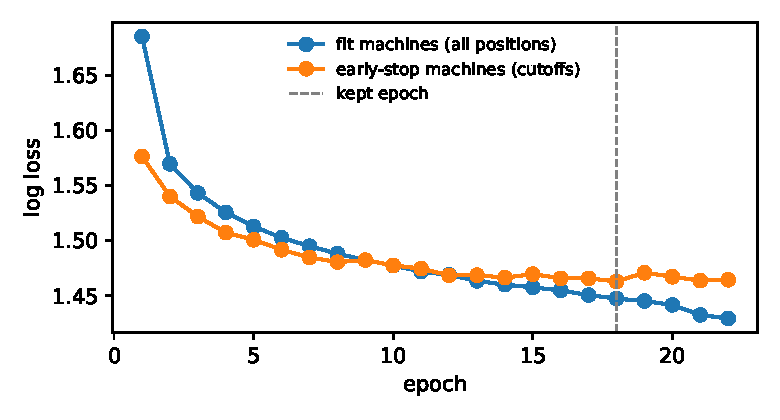
\includegraphics[width=0.62\linewidth]{figures/gru_learning_curve.pdf}
\caption{Training and early-stop log loss of the selected recurrent model.}
\end{figure}}{}

\IfFileExists{tables/gru_ablations.tex}{\begin{table}[htbp]
\centering\small
\begin{tabular}{@{}lrrr@{}}
\toprule
Change from selected GRU & Log loss & $\Delta$ & 95\% paired CI \\
\midrule
Remove time gaps & 1.4603 & +0.0081 & [+0.0024, +0.0137] \\
Remove sensors and missing flags & 1.4565 & +0.0043 & [-0.0011, +0.0097] \\
Remove categorical context & 1.4476 & -0.0046 & [-0.0094, +0.0005] \\
Last 16 events only & 1.5203 & +0.0681 & [+0.0598, +0.0768] \\
Last 64 events only & 1.4573 & +0.0051 & [+0.0003, +0.0098] \\
Add machine-relative sensors & 1.4526 & +0.0004 & [-0.0047, +0.0055] \\
Same model, different seed & 1.4473 & -0.0048 & [-0.0095, -0.0000] \\
No temperature scaling & 1.4521 & -0.0000 & [-0.0003, +0.0002] \\
\bottomrule
\end{tabular}
\caption{One change at a time around the selected recurrent model. Positive $\Delta$ means worse. Intervals resample validation machines.}
\end{table}
}{}
Retraining the selected model with a different seed changed validation loss by $-0.005$. We treat smaller effects as unreliable even when their machine-bootstrap interval excludes zero, because that interval does not include training randomness. History length had by far the largest effect. With only the last 16 events, loss rose by 0.068, while the last 64 events cost only about 0.005. Most of the useful context therefore lies within roughly the last 64 events, but a few events are not enough. Removing time gaps raised loss by 0.008 (95\% CI $[0.002, 0.014]$), the only input group whose removal clearly hurt, consistent with the importance of recency features in the classical model. Removing sensor inputs (+0.004, interval spanning zero) or categorical context ($-0.005$) changed loss by no more than the seed variation. This agrees with the classical result that sensor history adds little beyond the event stream. Machine-relative sensors (+0.0004) gave no gain. Temperature scaling fitted $T=1.01$ and changed loss by less than 0.0003, because the network was already calibrated: predictions made with 80--90\% confidence were correct 85\% of the time.

\IfFileExists{tables/gru_compare.tex}{\begin{table}[htbp]
\centering\small
\begin{tabular}{@{}lrrr@{}}
\toprule
Model (vs. selected GRU) & Log loss & $\Delta$ & 95\% paired CI \\
\midrule
LightGBM & 1.5193 & +0.0672 & [+0.0586, +0.0758] \\
Average of GRU and LightGBM & 1.4593 & +0.0071 & [+0.0027, +0.0115] \\
\bottomrule
\end{tabular}
\caption{Paired comparison on the shared validation cutoffs. The average is exploratory: equal weights, nothing tuned on validation.}
\end{table}
}{}
The selected GRU improves on the tuned LightGBM by 0.067 (95\% CI $[0.059, 0.076]$), larger than any single feature-group effect in the classical ablations. Averaging the two models' probabilities gave 1.459, which is 0.007 worse than the GRU alone. This suggests that LightGBM's hand-made counts and recency features add no information the GRU has not already learned from the raw sequence. A likely reason for the gain is that the GRU sees the exact order and timing of every event and is trained on about 95 prefixes per machine instead of 12 sampled cutoffs.


\subsection{Error analysis}
\IfFileExists{tables/classical_errors.tex}{For the selected classical model, prefixes of 90--129 events had validation log loss 1.532 (\(n=5294\)), versus 1.487 (\(n=1474\)) for 180--250 events. CONTROL\_ALERT had the largest class-average loss (4.626 over 88 examples). The class mix can differ across length buckets. The most common off-diagonal error was MAINTENANCE\_CHECK classified as VIBRATION\_WARNING (305 cases). The largest individual loss was 6.73, on a prefix of 106 events where the model assigned probability 0.00119 to CONTROL\_ALERT.
}{}
\todo{For the selected team model, report validation loss by event class and history length, with sample sizes. Discuss one high-loss error and one frequent confusion. Compare confidence with accuracy for the highest-confidence predictions and explain any evidence of overconfidence.}

\section{Generative sequence analysis}
\todo{Person C. Describe the generator inputs, prefix source, rollout horizon, number of prefixes, samples per prefix, sampling temperature and treatment of unavailable future measurements.}

\begin{table}[htbp]
\centering\small
\begin{tabularx}{\linewidth}{@{}lXX@{}}
\toprule
Diagnostic & Calculation & Result and interpretation \\
\midrule
Marginal behavior & Jensen--Shannon divergence on event frequencies & [Fill after running] \\
Local event order & Bigram/trigram comparison with matched real continuations & [Fill after running] \\
Diversity & Duplicate continuation rate or unique n-gram ratio & [Fill after running] \\
Timing (if generated) & Compare generated and real inter-event gaps & [Optional] \\
\bottomrule
\end{tabularx}
\caption{Planned diagnostics on generated and matched real continuations.}
\end{table}
\todo{Show representative real and sampled continuations from the same prefix. Discuss ordering, longer-range structure, diversity and possible memorization.}

\section{Conclusion and limitations}
\todo{State what improved next-event probabilities, what limitations remain in the prediction and generation findings, and what experiment would be most informative next. Address generalization beyond simulated systems.}


\clearpage
\begin{thebibliography}{9}
\bibitem{brief} AI2210 teaching team. \emph{EventFlow: Temporal Event Prediction}. Group project brief and baseline notebook.
\bibitem{lightgbm} G. Ke et al. LightGBM: A Highly Efficient Gradient Boosting Decision Tree. \emph{Advances in Neural Information Processing Systems}, 2017.
% Add the papers and technical resources actually used by the team.
\end{thebibliography}
\end{document}
